%----------------------------------------------------------------------------------------
% SECTION 2
%----------------------------------------------------------------------------------------

\section{Test Data}
\label{test_data}

There are a few sources for test-data of XPS-spectra. A main database was found on XPSlibrary, provided by TXL. The data was kindly sent to us in a readable text-format from B. Vincent Crist. From this database, > 400 spectra were used for the test dataset. In addition, the XPSSurfA on CMSS Hub from the Australian University La Trobe contains more than 1700 spectra of which $\approx$ 50 survey spectra were used for the evaluation of the model. The test data from the XPSSurfA-database is stored in web form, accessible as a zip-file, a script for automated data-acquisition was written, which can be found in Appendix \ref{xpslibrary_webscraper}.
Overall, we obtained $\nexperimentalspectra$ experimental spectra, consisting of $\nelementalspectra$ elemental spectra, $\nmultispectra$  multi-component (compound) spectra, and $\noxidespectra$ oxide spectra.
As spectra with identified two-layer systems were not found on publicly available databases, we assumed that pure elemental compounds are a two-layer system of the same compounds.

For multi-component spectra, $\nmultispectra$ experimental spectra were obtained from the libraries mentioned above. The spectra were renamed manually to facilitate the automatized label-readability, according to the scheme ${E_{1}\textunderscore X_{1} 	\textunderscore E_{2} 	\textunderscore X_{2} 	\textunderscore Filename}$, where $E_{1}$ is the first elemental component and $X_{1}$ is an integer providing its relative concentration. If experimental spectra had ratios indicated (eg. 25:75), these values were multiplied with the compounds. Thus, a file with the components \ch{Na2O-SiO2} (25:75) will be encoded with filename Na \textunderscore 50 \textunderscore O \textunderscore 175 \textunderscore Si \textunderscore 75 \textunderscore Filename. The one-hot encoding into vectors is then done with a function which parses the filename, it can be found in Appendix \ref{code:base}.

\subsection{Experimental depth profiles using sputtering}
To test the models' capabilities to predict depth profiles of spectra, sputtering experiments were conducted using Copper on Tungsten and Copper and Palladium.


\subsection{Data preprocessing}

As is typical for data acquired from laboratories, XPS data comes in various formats and measurement parameters. Apart from XPS-specific parameters, the resolution and the range mostly influence the evaluation of spectra with the deep-learning framework. Thus, an automated workflow for the spectra pre-processing is introduced to provide a valid input shape to the model.
Although most wide-survey spectra are measured with a comparable energy-range, it should be identical to the training data for prediction. Thus, any signal outside the specified binding energy range (0-1000 eV) is cut off and the discrete measurement points inside the range are interpolated (if less than 1024) or subsampled (if more than 1024) by using a cubic-spline sampling method to match 1024 points. The most common format is the VAMAS format, established in 1988 by Dench et al \cite{dench_vamas_1988}. It has been slightly modified to the ISO Standard \cite{1400-1700_iso_nodate}(ISO 14976:1998) and thus is very popular and readable by most XPS applications. A python library found on the python package index PyPi called vamas \cite{krinninger_vamas_nodate} was used under slight adaptations due to version updates of related packages. It allows reading and extracting data from Vamas files in a object-oriented manner.
Most experimental files obtained contain so-called blocks, which are sub-experiments on the same sample. In the different blocks, we usually find different analysis regions, such as a specific region for an atomic orbital, or the survey spectrum.

\begin{figure}
    \centering
    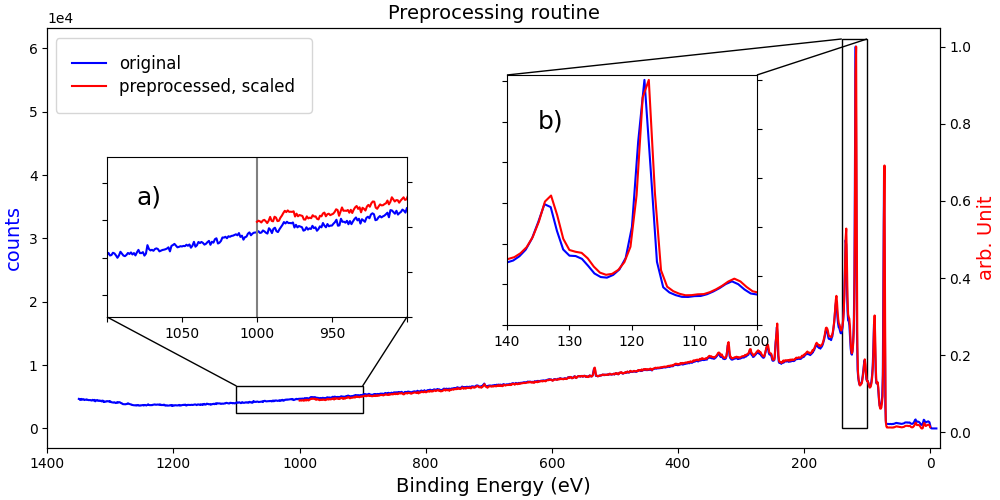
\includegraphics[width=\textwidth]{Figures/preprocessing_routine.png}
    \caption{Preprocessing routine result of experimental spectra (Aluminum). Experimental spectrum before (blue) and after (red) the preprocessing routine. Spectra are cut off at 1000 eV as shown in a) and at 0 eV. Slight changes to the peak shape are a result of the resampling method as shown in b).}
    \label{fig:preproc_routine}
\end{figure}

The preprocessing results of a selection of experimental spectra were then assessed, as shown in Figure \ref{fig:ex_vs_sim}.

\begin{figure}
    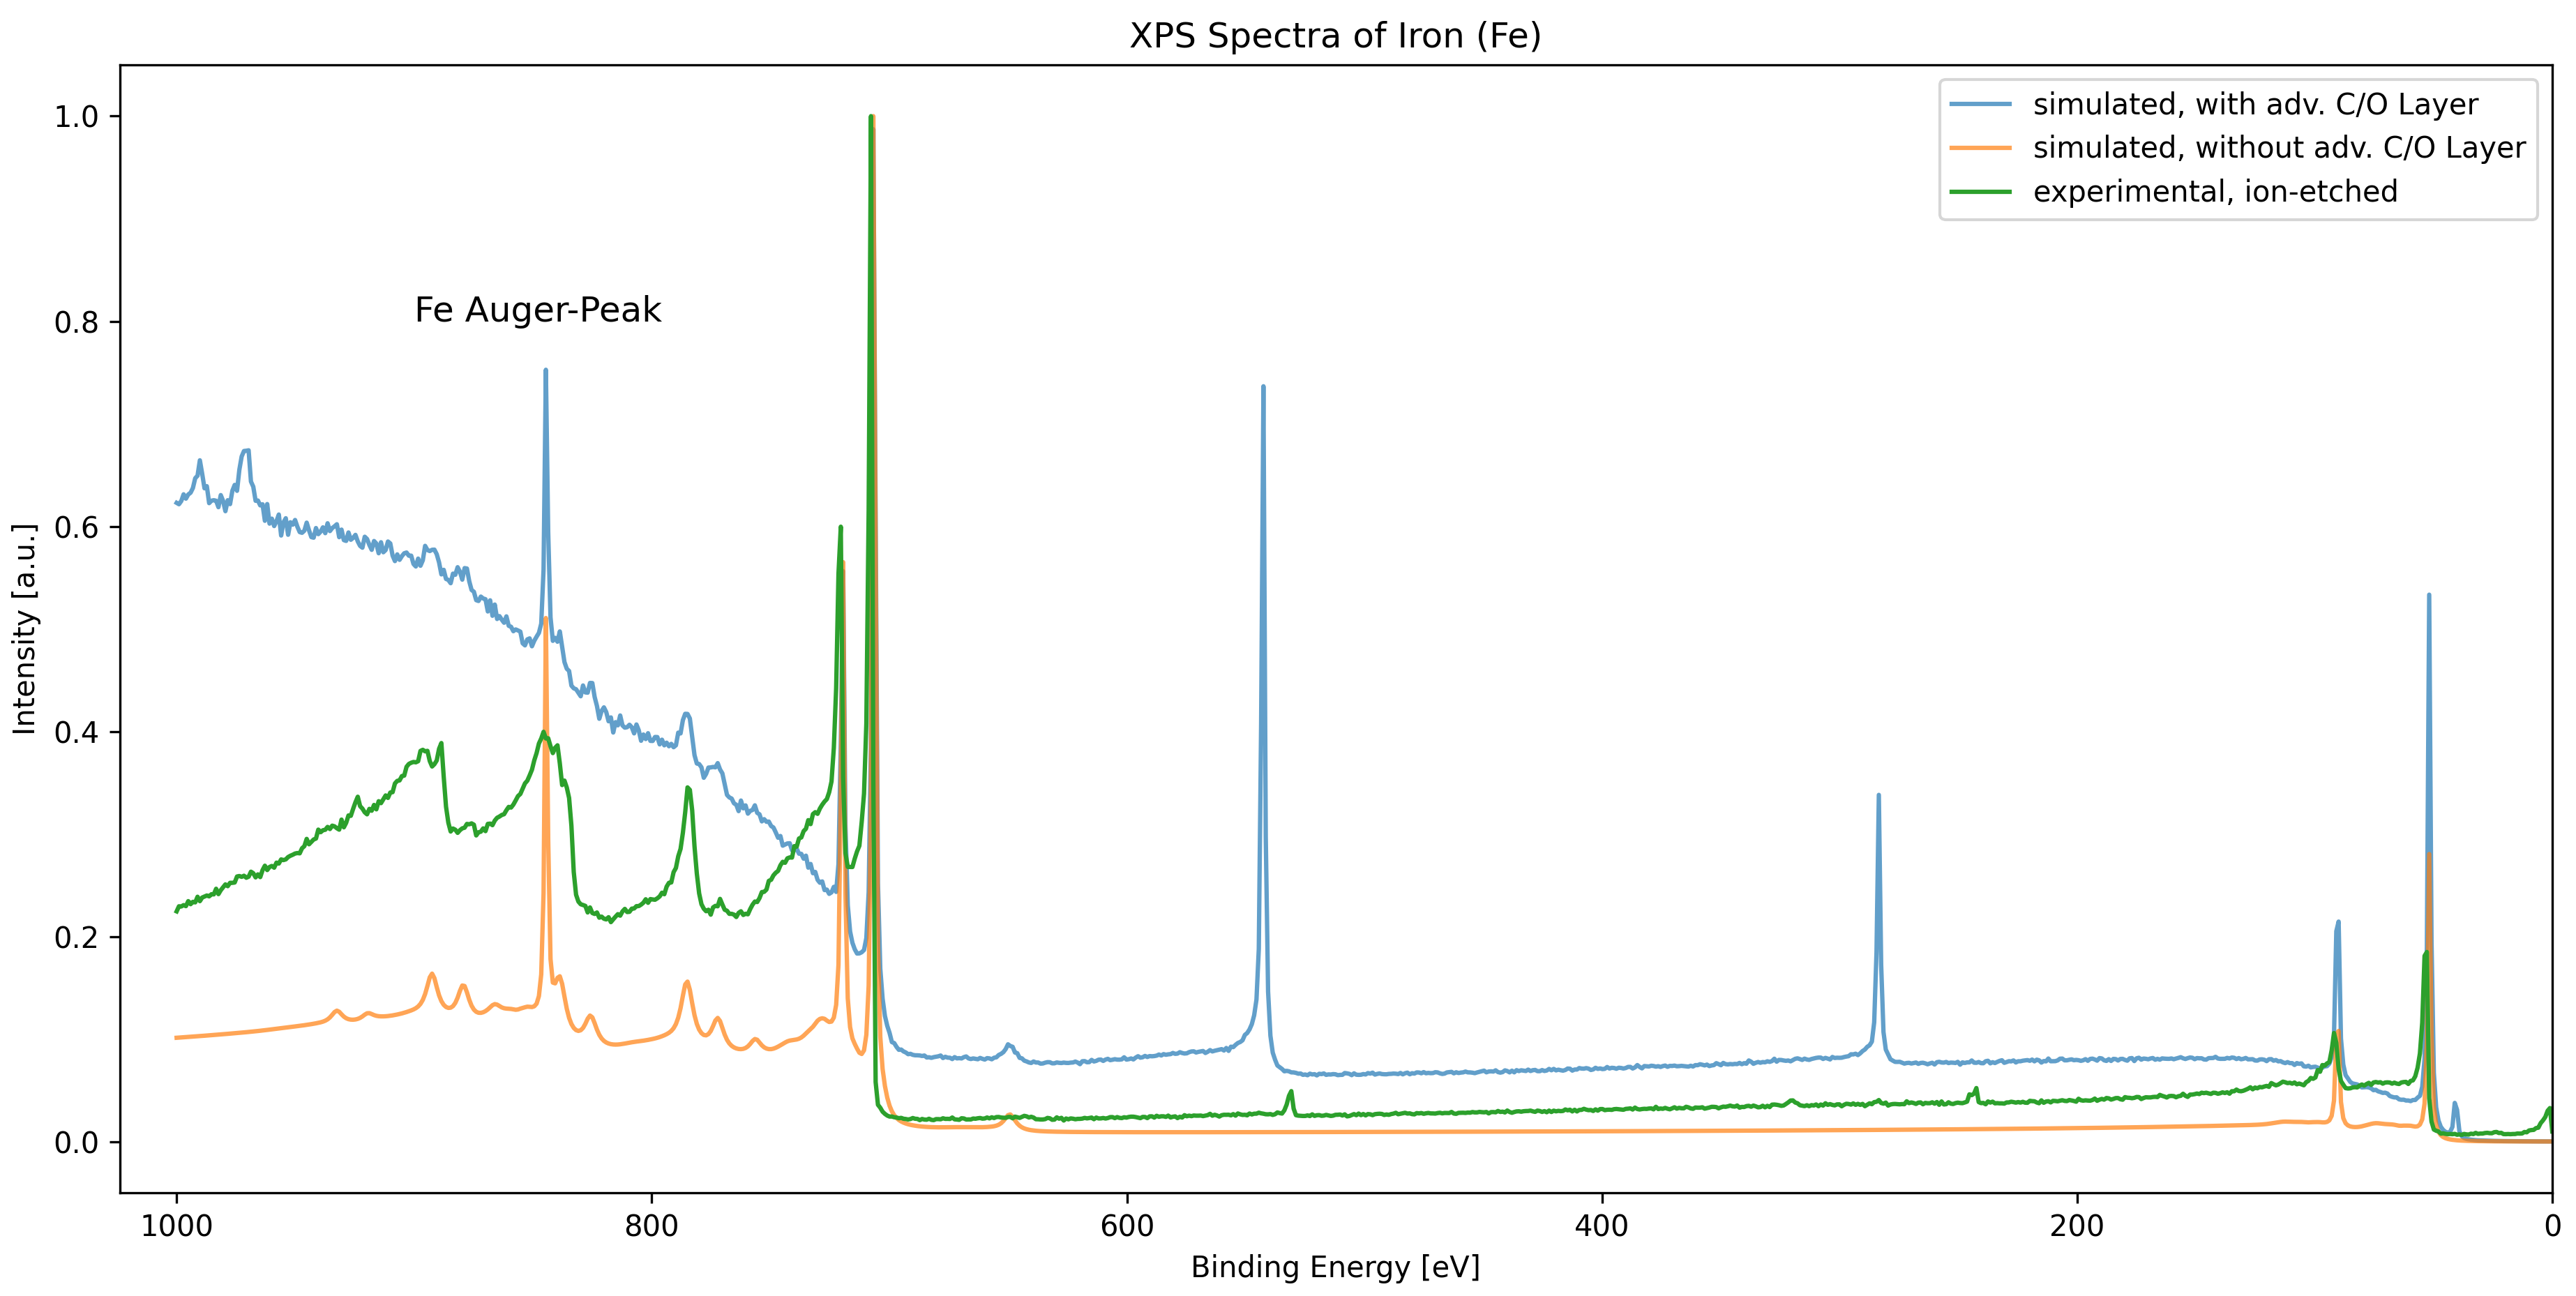
\includegraphics[width=\textwidth]{Figures/Fe_XPS.png}
    \caption{Comparison of experimental \& preprocessed vs simulated spectra of elemental iron}
    \label{fig:ex_vs_sim}
    \centering
\end{figure}

The python module used to preprocess the experimental data can be found in \nameref{AppendixA}.